\documentclass[12pt]{article}


% Language setting
% Replace `english' with e.g. `spanish' to change the document language
\usepackage[english]{babel}

% Set page size and margins
% Replace `letterpaper' with `a4paper' for UK/EU standard size
\usepackage[letterpaper,top=2cm,bottom=2cm,left=2cm,right=2cm,marginparwidth=2cm]{geometry}

\usepackage{listings}

% Useful packages
\usepackage{amsmath}
\usepackage{graphicx}
\usepackage[colorlinks=true, allcolors=blue]{hyperref}

\title{Polytechnique Montreal \\
LOG8415: Lab 1\\
Cluster Benchmarking using EC2 Virtual
Machines and Elastic Load Balancer (ELB)}

\author{Line Ghanem - 1728134\\Zineddine Aliche - 1949905\\
Mohammed Ramzi Bouthiba - 2065386\\Axelle Pagnier - 2164162}

\begin{document}
\maketitle

\begin{abstract}
In this	assignment,	we	create	two	clusters of	EC2 virtual	machines and use	a load	balancer	to	distribute	workloads	and	perform	extensive	benchmarking	on	those instances.\newline
First, we will explain the overall architecture that is going to be deployed using Amazon Web Services. Then we will talk about the flask application that we deployed on the EC2 instances. After that, we will discuss the performance metrics of the instances and the load balancer that we retreived using CloudWatch.	Finally, we will provide an automated solution to do the set up and the benchmarking.
\end{abstract}

\section{Setting Up the Environment}

In this section, we discuss the steps that lead to the creation of the EC2 instances, target groups and the load balancer in order to prepare our environment for benchmarking. Figure 1 illustrates the process we followed to set up the environment.\vspace{1em}

We start with the creation of a custom core virtual networking with the Amazon virtual Private Cloud (VPC) service. The goal is to have complete control of the virtual network environment, including resource placement, connectivity, and security.\vspace{1em}

The second step consists of the creation of an internet gateway which allows to ensure the communication between our resources in the VPC and the internet.\vspace{1em}

The creation of a custom VPC needs to have custom subnets, for this we have created two different ones, one for each availability zone ('us-east-1a' and 'us-east-1b'). However, before creating the subnets we have established a routing table because each subnet in VPC must be associated with a routing table, which controls the network traffic routing for the subnet.\vspace{1em}

To secure the instances that we are going to generate, we have created a security group which acts as a virtual firewall for our EC2 instances and which contains a set of rules that filter incoming and outgoing traffic. We allowed HTTP and SSH connections from everywhere (0.0.0.0/0)\vspace{1em}

Once all the steps discussed above have been completed, we proceed to the creation of our EC2 instances. In total \textbf{9} instances have been created in the same region \textbf{'us-east-1'}, with two different types of instances: \textbf{'m4.large'} and \textbf{'t2.large'}. Five (05) of the instances are of type 'm4.large' in the availability zone 'us-east-1a' and four (04) are of type 't2.large' in the availability zone 'us-east-1b'.\vspace{1em}

In order to group the instances to form the clusters, two target groups have been created, the first with the instances of type 'm4.large' and the second with the type 't2.large'.\vspace{1em}

The final step for setting up the environment is the creation of the load balancer, which will manage the request traffic sent to our clusters, the type of load balancer used is \textbf{Application Load Balancer} (ALB) that operate at layer 7 (application layer). This load balancer will serve	 as	 the	 single	 point	 of	 contact	 for	 clients.	 The	 load	 balancer	 distributes	 incoming	application	traffic	across	multiple	our	EC2	instances,	in the two	availability	zones that we created.	This	increases	the	availability	of	our	flask application that we will discuss in the next section.

\begin{figure}[h]
  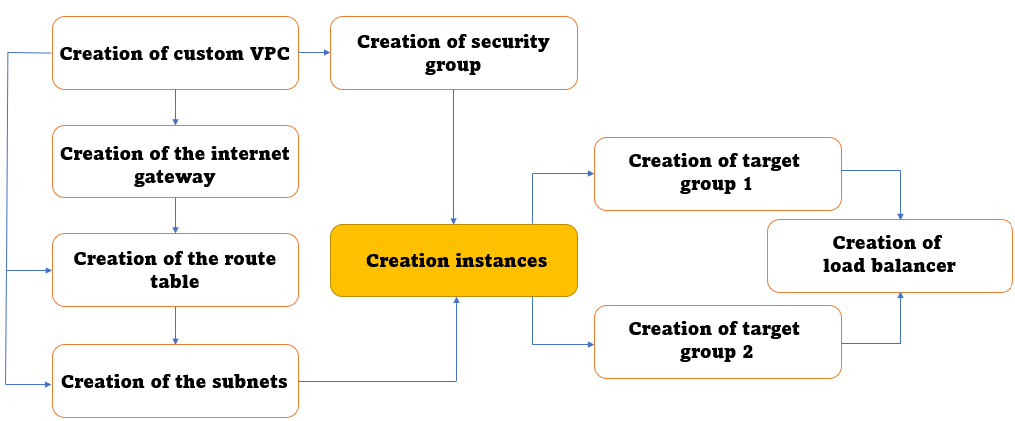
\includegraphics[width=\linewidth]{Environment_setup.png}
  \caption{Setting up the environment.}
  \label{fig:boat1}
\end{figure}

\section{Deploying the Flask Application}

To deploy the flask application we created an ssh connection to each of the instances using the python library paramiko \cite{paramiko}.\vspace{1em}

Once the connection was established using the key pair, we ran a bash script that would set up the environment for python and flask, add the code for the application and then deploy it on port 80 of each instance.\vspace{1em}
To deploy our small app we simply used the following command:
\begin{lstlisting}[language=Bash]
nohup sudo flask run --host=0.0.0.0 --port=80 1>/dev/null 2>/dev/null &
\end{lstlisting}\vspace{1em}

To speed up the deployment process, we used multi-threading. Instead of waiting for each instance to install python and flask and deploy the app on port 80, we used 9 threads to connect to each instance and send the commands to set up the environment simultaneously. This sped up the deployment process significantly.\vspace{1em}

The bash command \emph{nohup}, keeps any process that is started after it running in the background so that we can exit the command line safely without stopping our small app. For example, given an instance with a public ip: 111.111.111, the user can go to the following url: http://111.111.111:80 and the app should be running. The page should simply display a message:\vspace{1em}

\emph{Your small app is working on instance id: instance\_id}.\vspace{1em}

It is important in the following assignment to know which instance is responding since we will try to connect to the website using the load balancer. 

\section{Benchmarking}

In order to test the performance of our system. we created a python script that sends 2500 GET requests to the load balancer DNS address. Then, the load balancer distributes the workload on the 9 instances according to its load balancing algorithm.\vspace{1em}

We separated the GET requests into two threads. Thread 1 sends 1000 GET requests in one go, and Thread 2 sends 500 GET requests, waits one minutes, then sends another 1000 GET requests. The two threads run concurrently.\vspace{1em}

To analyse the performance of the system, we used Amazon CloudWatch to retreive the metrics. CloudWatch monitors our AWS resources in real time.\vspace{1em}

First we activated detailed monitoring for all the EC2 instances in order to have a period of 1 minute between each datapoint. After that we send the aforementioned GET requests. After finishing sending the requests to the load balancer, we fetch two important metrics to analyze. the first metric is CPU\_Utilization (The percentage of allocated EC2 compute units that are currently in use on the instance) and the second one is NetworkIn (The number of bytes received by the instance on all network interfaces).\vspace{1em}

After collecting those metrics, we store them in a .json file in order to plot them using matplotlib (a plotting library for python) and analyze them.\vspace{1em}

The following graphs are an example of the metrics that we retrieved after setting up the environment and sending the GET requests.\vspace{7em}

\begin{figure}[htbp]
\centering
  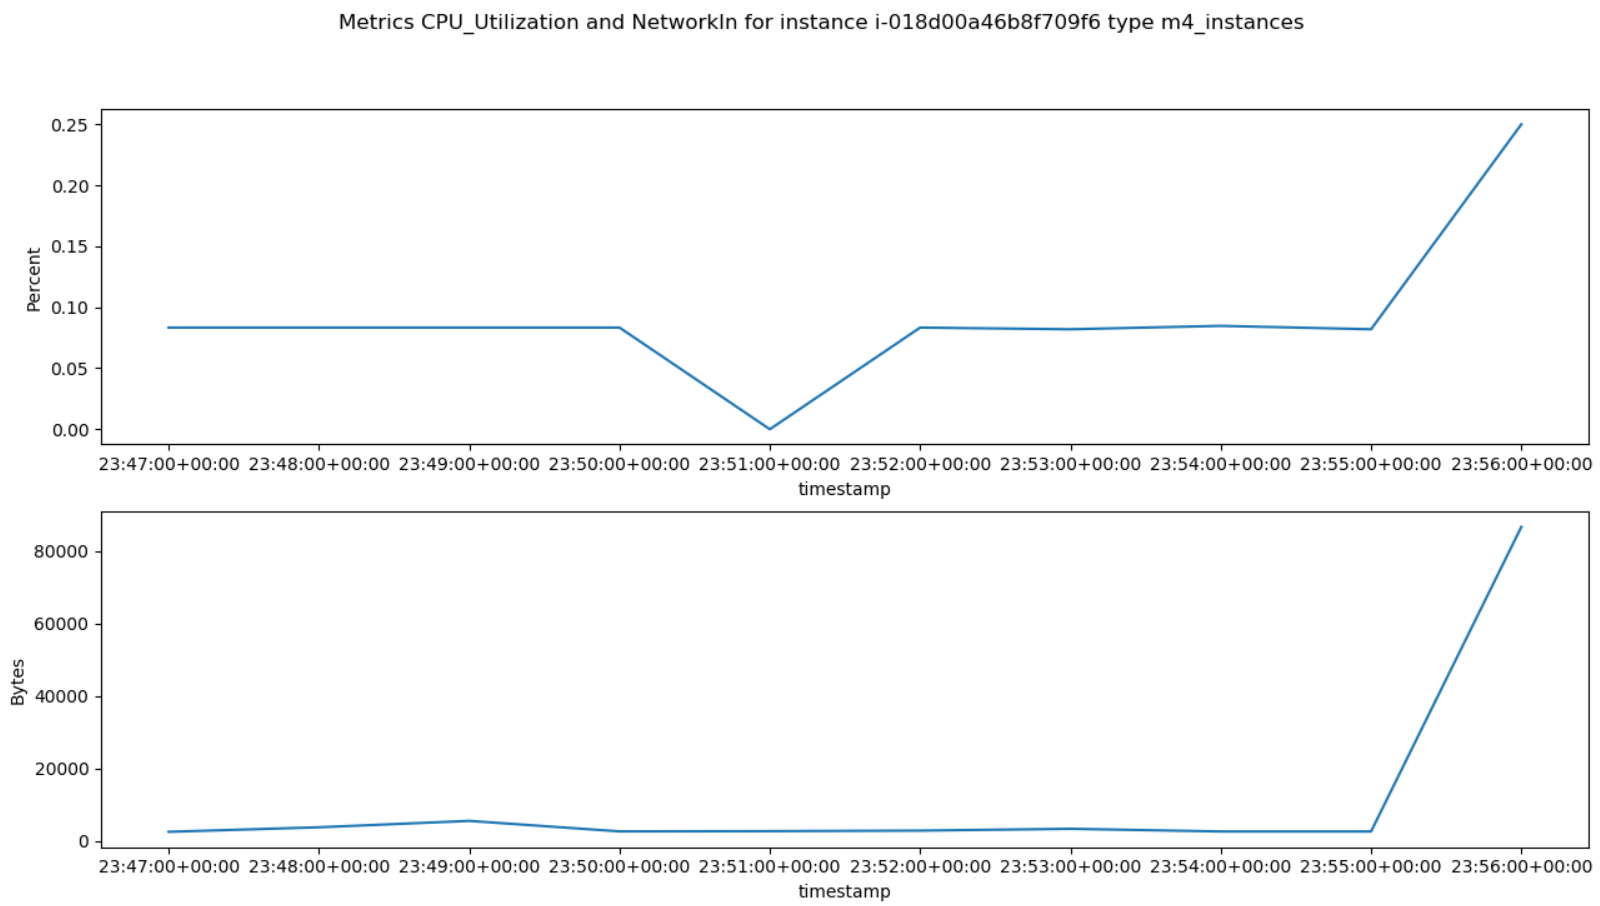
\includegraphics[height=300px]{Capture1.png}
  \caption{Performance metrics of instance with ID: i-018d00a46b8f709f6}
\end{figure}

\begin{figure}[htbp]
\centering
  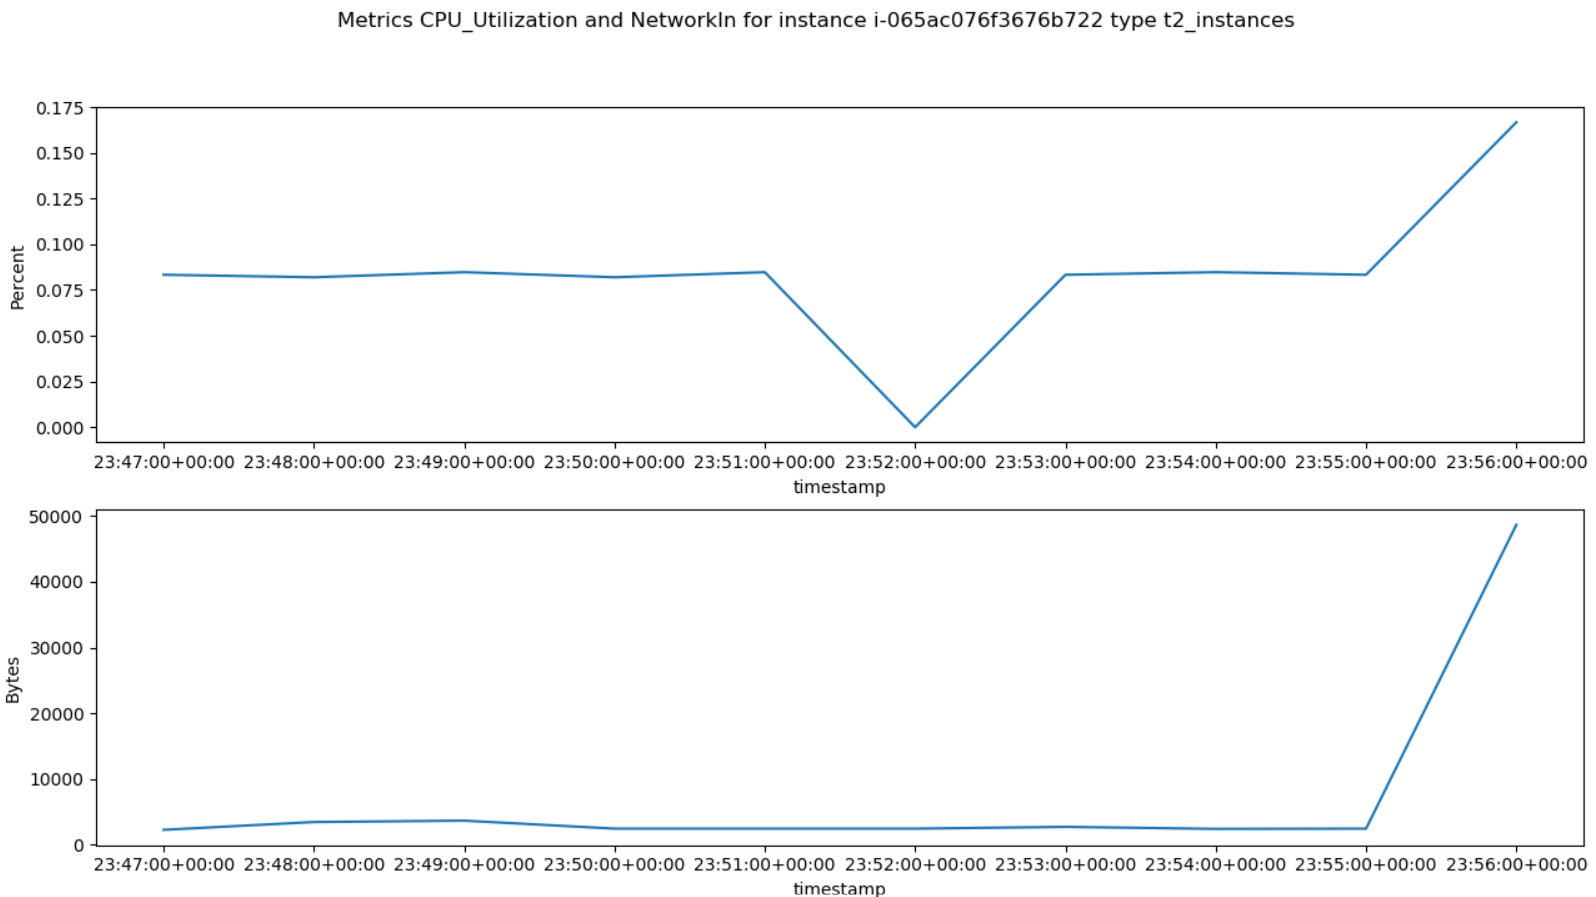
\includegraphics[height=300px]{Capture2.png}
  \caption{Performance metrics of instance with ID: i-074b2a94d5e893130}
\end{figure}

By looking at the graphs of the two different EC2 instances, we can see that our load balancer did a great job at distributing the workloads amongst the instances since the NetworkIn metric (the bottom graph for each instance) follow the same trend at any given time.

\section{Instructions to run the code}

To reproduce the experiment, all you have to do is download the main.sh file and run it on your local computer. Make sure you have an internet connection and an AWS account. \\
Once the repository is cloned, don't forget to : \\
1. Set up your AWS credentials file (~/.aws/credentials). \\
2. Put your SSH key (.pem file) inside the /src folder.

\section{Conclusion}

According to the performance metrics that we got, we can conclude that our system works as expected. The EC2 instances serve the web app correctly, the load balancer distributes the workload \emph{efficiently} amongst the instances across the two different availability zones.

\begin{thebibliography}{9}
\bibitem{paramiko}
Paramiko, Availible online: https://www.paramiko.org/, Accessed: Oct. 2022. 
\end{thebibliography}

\end{document}
